%Chapter 1

\renewcommand{\thechapter}{1}

\chapter{Introduction}
% Going for about 5 pages or so here.

Eighteen years ago the Oceanstore paper~\cite{oceanstore} presented a vision for a data utility infrastructure that spanned the globe.
The economic model was that of a cooperative utility provided by a confederation of companies that could buy and sell capacity to directly support their users, with regional providers like airports and cafes installing servers to enhance performance for a small dividend of the utility.
This economic model meant that Oceanstore's requirements centered around an untrusted infrastructure to support nomadic data: connectivity, security, durability, and location agnostic storage.
To meet these requirements, the Oceanstore architecture was composed of two tiers: pools of byzantine quorums that made localized consistency and placement decisions, along with an optimistic dissemination tree layer that moved data between quorums as correctly as possible without providing guarantees.
This architecture, along with a reliance on encryption and key-based access control, could facilitate grid computing storage, a truly decentralized and independent participation of heterogenous computational resources across the globe~\cite{grid_computing}.

Unforeseen by Oceanstore, however, was a fundamental shift in how companies and users accessed computing infrastructure.
Improvements in virtualization management~\cite{eucalyptus} and later container computing~\cite{docker} allowed big internet companies to easily lease their unused computational resources and disk capacity to application developers, making cloud computing~\cite{cloud_computing} rather than independent hardware purchasing and hosting the norm.
Furthermore, from smarter phones to tablets and netbooks that do not have large disk capacities, user devices have become increasingly mobile; from photos to email and contacts, most user data is now stored in cloud silos.
The cloud economy means that there exists a \emph{trusted infrastructure} of virtual resources that span globe, provisioned by a single provider as shown in Figure~\ref{fig:ch01_cloud_data_centers}.

\begin{figure}
    \begin{center}
        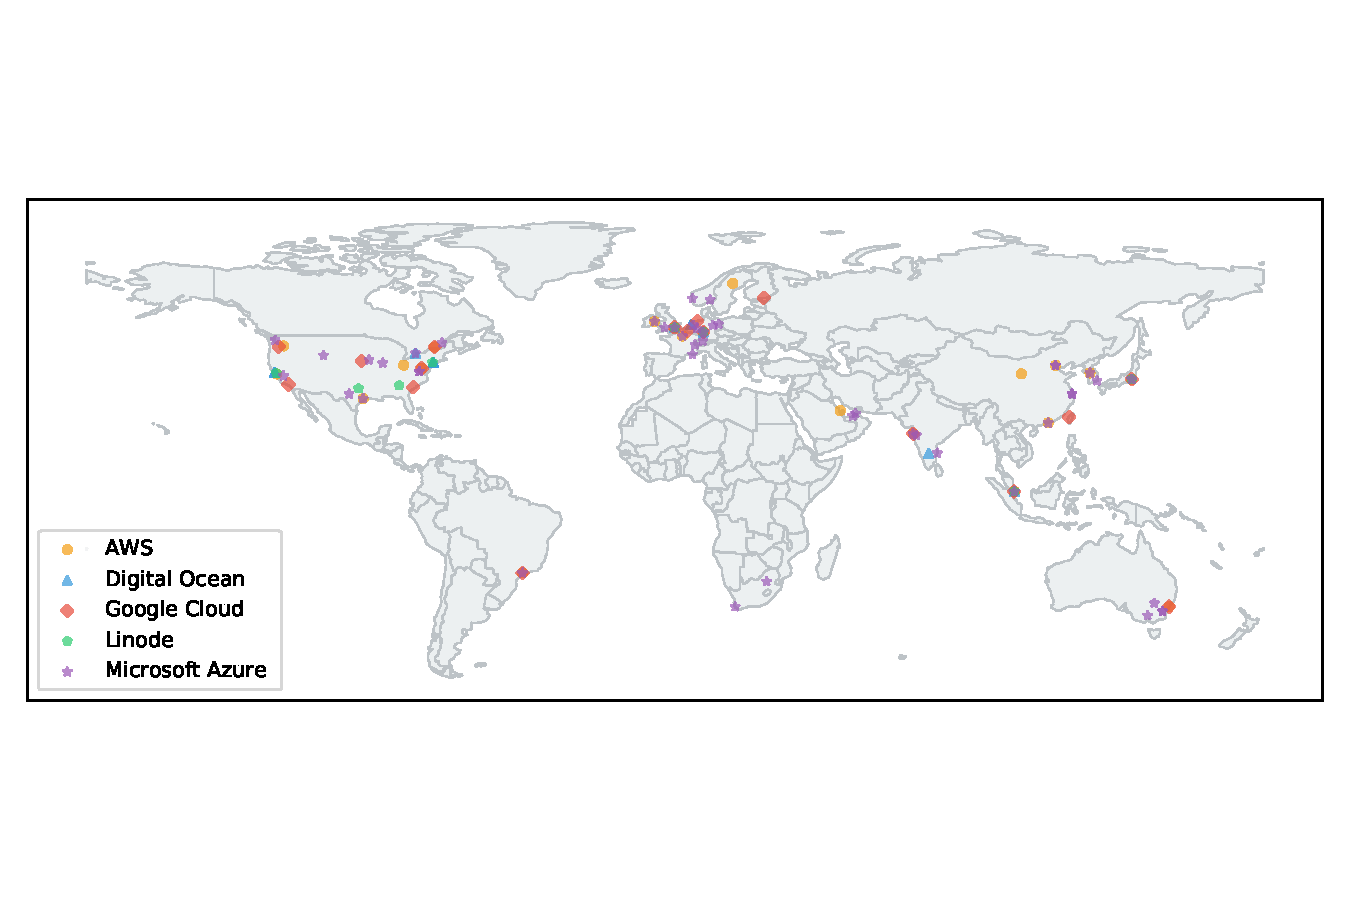
\includegraphics[width=5in]{figures/ch01_cloud_data_centers.pdf}
    \end{center}
    \renewcommand{\baselinestretch}{1}
    \small\normalsize

    \begin{quote}
        \caption[Global Data Centers of Cloud Providers]{Data center locations of popular cloud providers span the globe.}
        \label{fig:ch01_cloud_data_centers}
    \end{quote}
\end{figure}
\renewcommand{\baselinestretch}{2}
\small\normalsize

% Do better at this paragraph
So what does this mean for the requirements and assumptions of Oceanstore?
First, the strict requirements for security that meant per-user encryption and byzantine agreement between untrusted servers can be relaxed to application and transport-level encryption and non-byzantine consensus supported by authenticated communication.
Second, the requirements for performance have dramatically increased as ubiquitous computing has become the norm and as more non-human users are participating in networks.
Increased capacity, however, cannot come at the cost of correctness or consistency, and the increased rate of requests means that asynchronous commits and conflict resolution become far more difficult.
For these reasons, we believe that a vision for an Oceanstore today would focus on \emph{consistency} rather than security.

% How do we transition to this paragraph?
Consistent behavior in distributed systems becomes increasingly complex to implement and reason about as the system size grows and requires increased coordination.
In 2021, Cisco forecasts over 25 billion devices will contribute to 105,800 GBps of global internet traffic, 26\% of which will be file sharing and application data, and 51\% of which will originate from machine to machine-to-machine applications \cite{cisco_internet_trends}.
New types of networks including sensor networks, smart grid solutions, self-driving vehicle networks, and an internet of things will mean an update model with many publishers, few subscribers, and increasingly distributed accesses.
To support this growth and facilitate speed, traffic is consistently moving closer to the edge; Cisco predicts that cross-country delivery will drop from 58\% of traffic in 2016 to 41\% in 2021 and that metro delivery will grow from 22\% to 35\%.
Localization means that the cloud will be surrounded by a fog of devices that participate in systems by contributing data storage and computation to an extent greater than access-oriented clients might.

% Do I need to make this point sooner?
Based on these trends and inspired by the work of Oceanstore, we propose that a consistent planetary-scale data storage system would be made up of a two tier architecture of both cloud and fog infrastructure.
The first tier, in the cloud, would be a strong consistency, fault tolerant and highly resilient geo-replicated consensus backbone: \emph{hierarchical consensus}.
The second tier, via the fog, would be a high availability heterogenous network with a hybrid consistency model: \emph{federated consistency}.
Such a system would be difficult to manually manage, therefore the system would also have to automatically monitor and adapt to changes in access patterns and node and network availability during runtime.
We believe that the combination of hierarchical consensus, federated consistency, and adaptive monitoring lay out a foundation for truly large scale data storage systems that span the planet.

The contributions of this dissertation are therefore as follows:

\begin{enumerate}
    \item We present the design, implementation, and evaluation of hierarchical consensus, a consensus protocol that can scale to dozens or hundreds of replicas across the wide area.
    \item We also investigate the design and implementation of federated consistency, a hybrid consistency model that allows strong, consensus-based systems to integrate with eventually-consistent, highly available replicas and evaluate it in a simulated heterogenous network.
    \item We show the possibilities for machine learning-based system adaptation with a reinforcement learning approach to anti-entropy synchronizations based on accesses.
    \item We validate our system by describing the implementation of a planetary-scale key-value data store and file system using both hierarchical consensus and federated consistency.
\end{enumerate}


% Contributions:
%     Design, implementation, and evaluation of hierarchical consensus
%     Design, implementation, and evaluation of federated consistency
%     Design, implementation, and evaluation of bandit-based anti-entropy
%     Design and implementation of planetary-scale key/value store
%     Design and implementation of a planetary-scale file system
%     Description and discussion of distributed systems in the very wide area
%     Description and discussion of dependent scaling of consensus algorithms

The rest of this dissertation is organized as follows.
In the next chapter we will more thoroughly describe the motivations and challenges of building geo-replicated data systems as well as explore case-studies of existing systems.
Next, we will focus on the core backbone of our system: hierarchical consensus and describe a globally fault tolerant approach to managing accesses to objects in the wide area.
Using hierarchical consensus as a building block, we will next describe federated consistency and how a hybrid, heterogenous consistency model in the fog interacts with the cloud consensus tier.
At this point we will have enough background to introduce our system implementation and describe our file system and key-value store.
From there, we will explore learning systems that monitor and adapt the performance of the system at runtime, before concluding with related work and a discussion of our future research.
